\documentclass[12pt,a4paper]{report}
\usepackage[utf8]{inputenc}
\usepackage[english,russian]{babel}
\usepackage{indentfirst}
\usepackage{pdfpages}
\usepackage{titlesec}
\usepackage{listings}
\usepackage{amsmath}

% Вставка картинки
\usepackage{graphicx}
\graphicspath{{schemes/}}
\DeclareGraphicsExtensions{.pdf,.png,.jpg}

\usepackage[tableposition=top,singlelinecheck=false]{caption}

\usepackage[14pt]{extsizes}

\newcommand{\hsp}{\hspace{20pt}}
\titleformat{\chapter}[hang]{\large\bfseries}{\thechapter{. }}{0pt}{\large\bfseries}
\titlelabel{hlabel-formati}
\titlespacing{\chapter}{42pt}{-20pt}{12pt}
\titleformat{\section}[hang]{\large\bfseries}{\thesection{. }}{0pt}{\large\bfseries}
\titlespacing{\section}{42pt}{12pt}{5pt plus 5pt}

% Отступ абзаца
\usepackage{indentfirst}
\setlength{\parindent}{1.5cm}

% Межстрочный интервал
\usepackage{setspace}
\onehalfspacing % интервал 1.5


\usepackage{csvsimple}

\bibliography{biblio}
\lstset{frame=none, tabsize=4}

\usepackage[left=3cm, right=1cm, top=2cm, bottom=2cm]{geometry}

\AtBeginDocument{%
	\renewcommand\contentsname{Содержание}
}

\begin{document}
% Титульник
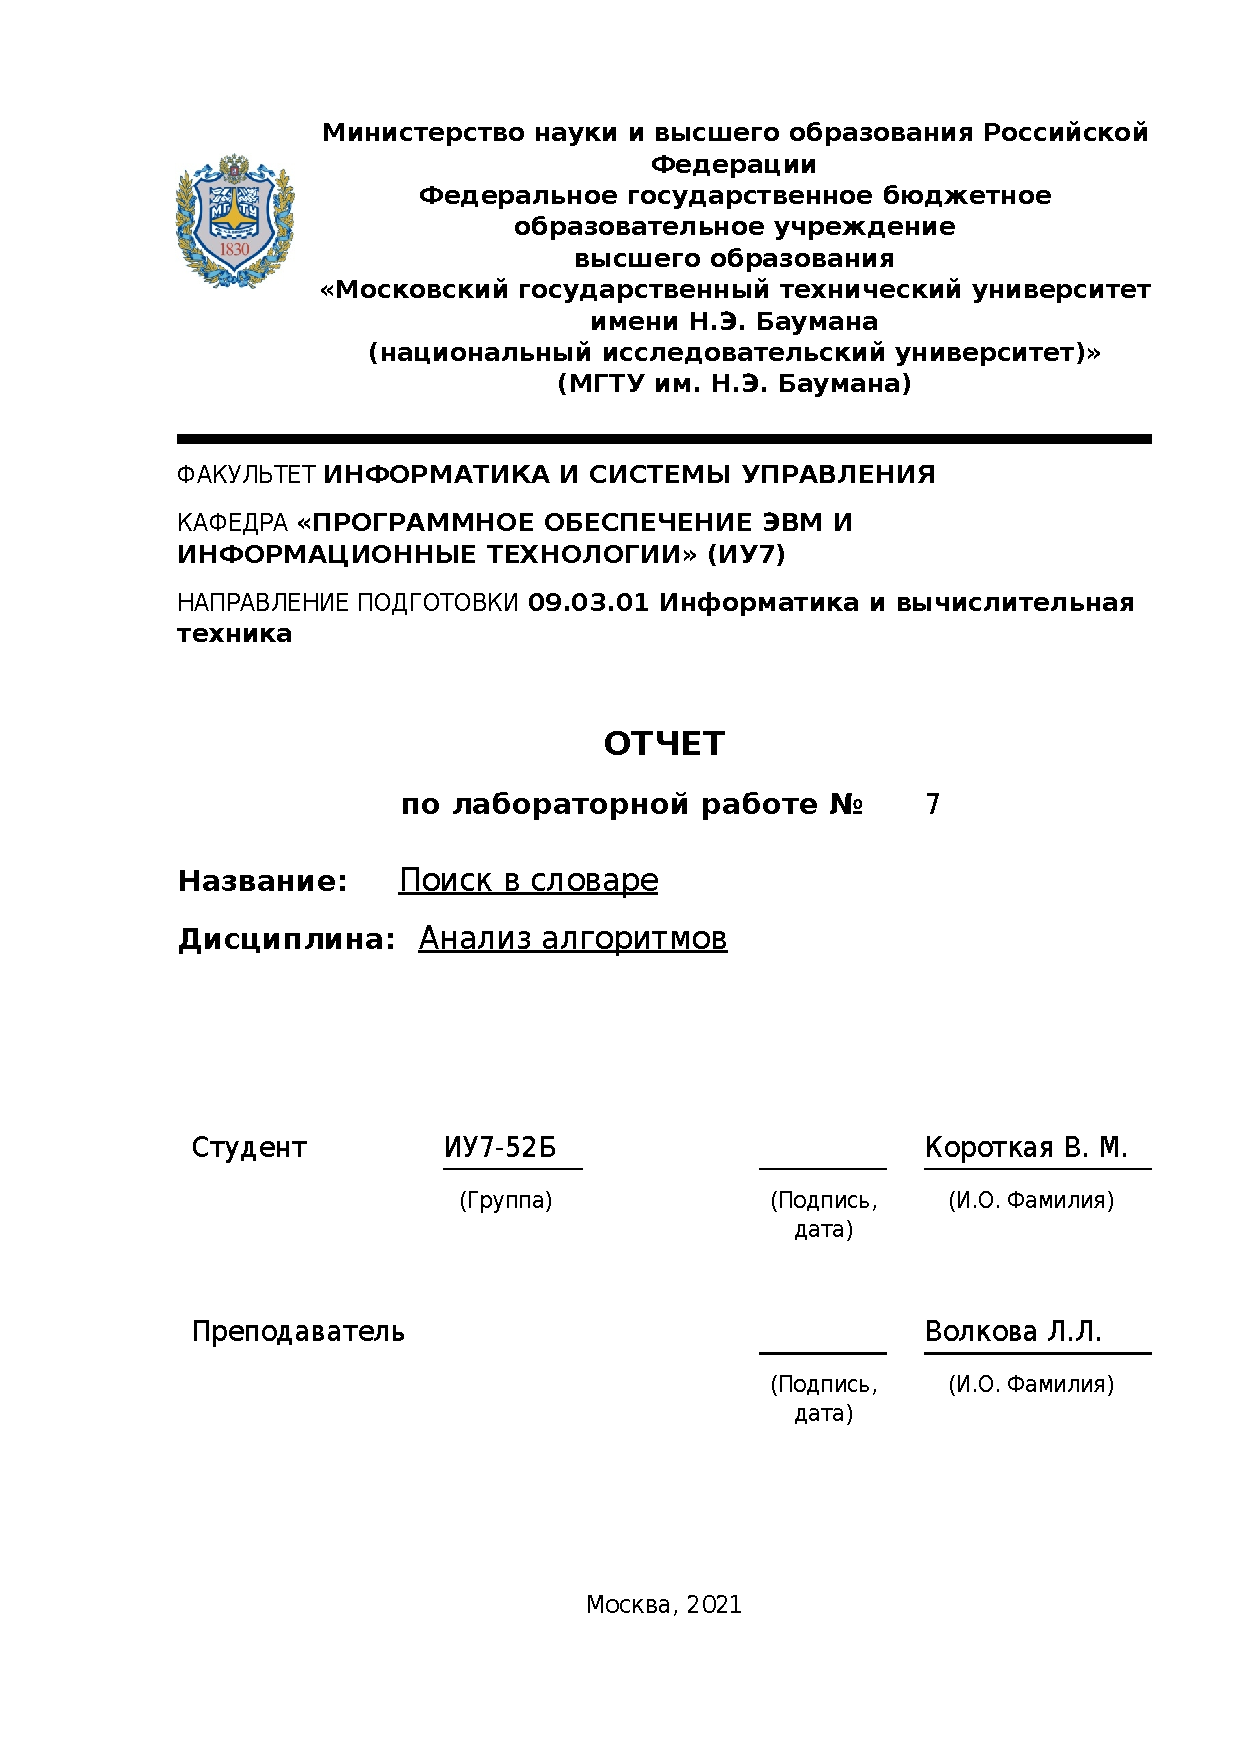
\includepdf[pages=1]{titul.pdf}
% Оглавление
\tableofcontents

	
\newpage
\chapter*{Введение}
\addcontentsline{toc}{chapter}{Введение}


Ассоциативный массив — абстрактный тип данных (интерфейс к хранилищу данных), позволяющий хранить пары вида «(ключ, значение)» и поддерживающий операции добавления пары, а также поиска и удаления пары по ключу:

\begin{itemize}
	\item INSERT(ключ, значение)
	\item FIND(ключ)
	\item REMOVE(ключ)
\end{itemize}

Предполагается, что ассоциативный массив не может хранить две пары с одинаковыми ключами.

В паре (k, v) значение v называется значением, ассоциированным с ключом k. Где k — это key, a v — value. 

Операция FIND(ключ) возвращает значение, ассоциированное с заданным ключом, или некоторый специальный объект UNDEF, означающий, что значения, ассоциированного с заданным ключом, нет. Две другие операции ничего не возвращают (за исключением, возможно, информации о том, успешно ли была выполнена данная операция).

Ассоциативный массив с точки зрения интерфейса удобно рассматривать как обычный массив, в котором в качестве индексов можно использовать не только целые числа, но и значения других типов — например, строки.

Поддержка ассоциативных массивов есть во многих интерпретируемых языках программирования высокого уровня, таких, как Perl, PHP, Python, Ruby, Tcl, JavaScript и других. Для языков, которые не имеют встроенных средств работы с ассоциативными массивами, существует множество реализаций в виде библиотек.

Примером ассоциативного массива является телефонный справочник: значением в данном случае является совокупность «Ф. И. О. + адрес», а ключом — номер телефона, один номер телефона имеет одного владельца, но один человек может иметь несколько номеров.

Три основных операции часто дополняются другими, наиболее популярные расширения:


\begin{itemize}
	\item CLEAR — удалить все записи,
	\item EACH — «пробежаться» по всем хранимым парам,
	\item MIN — найти пару с минимальным значением ключа,
	\item MAX — найти пару с максимальным значением ключа.
\end{itemize}

В последних двух случаях необходимо, чтобы на ключах была определена операция сравнения.

Целью данной лабороторной работы является изучение способа эффекливного по времени и памяти поиска по словарю. Для достижения данной цели необходимо решить следущие задачи:

\begin{itemize}
	\item исследовать алгоритмы поиска по словарю;
	\item привести схемы рассматриваемых алгоритмов;
	\item провести тестирование работы алгоритмов в лучшем, худшем и произвольном случае;
	\item провести замеры процессорного времени работы алгоритмов поиска по словарю для каждого ключа и для отсутствующего ключа, вывести минимальное, максимальное и среднее время поиска ключа;
	\item сделать вывод о проделанной работе и описать в отчете.
\end{itemize}

\newpage
\chapter{Аналитическая часть}

В данном разделе приведены теоритические сведения о рассматриваемых алгоритмов.


\section{Алгоритм полного перебора}

Идея алгоритма заключается в том, что поиск заданного элемента из множества происходит непосредственно 
сравниванием каждого элемента этого множества с искомым, до тех пор, пока искомый не найдётся или множество
не закончится. 

Сложность алгоритма линейно зависит от объёма словаря, а время может стремиться к экспоненциальному времени 
работы. 


\section{Алгоритм бинарного поиска}

Данный алгоритм содержит в себе идею, которая заключается в том, что берётся значение ключа из середины словаря и 
сравнивается с данным. 
Если значение меньше (в контексте типа данных) данного, то продолжается поиск в левой части словаря, при обратном случае - в правой. 
На новом интервале также берётся значение ключа из середины и сравнивается с данным. 
Так продолжается до тех пор, пока найденное значение ключа не будет равно данному.

Поиск в словаре с использованием данного алгоритма в худшем случае будет иметь трудоёмкость $O(log_{2}N)$, что быстрее 
поиска при помощи алгоритма полного перебора. 
Но стоит учитывать, что алгоритм бинарного поиска работает только для заранее отсортированного словаря. 

В случае большого объёма словаря и обратного порядка сортировки, может произойти так, что алгоритм полного перебора 
будет эффективнее по времени.  


\section{Алгоритм частного анализа}


Идея алгоритма заключается в составлении частотного анализа. Чтобы провести частотный анализ, необходимо взять
первый элемент каждого значения в словаре по ключу и подсчитать частотную характеристику, т.е. сколько раз этот 
элемент встречается в качестве первого элемента. По полученным значениям словарь разбивается на сегменты так, 
что все элементы с одинаковым первым элементом оказываются в одном сегменте.

Далее сегменты упорядочиваются по значению частотной характеристики таким образом, чтобы элементы с наибольшей 
частотной характеристикой был самый быстрый доступ.

Далее каждый сегмент упорядочивается по значению. Это необходимо для реализации бинарного поиска, который 
обеспечит эффективный поиск в сегменте при сложности $O(N log N)$.


\section{Описание словаря}

В данной работе словарь представляет собой базу данных имён и имеет вид \{key: number, name: string\}. Поиск 
будет реализован по полю key.

\section*{Вывод}

В данной работе стоит задача реализации поиска в словаре, были рассмотрены алгоритмы реализации данного поиска.

Входными данными являются:

\begin{itemize}
	\item словарь записей, вида \emph{ {username:string, password:string}};
	\item ключ для поиска по словарю.
\end{itemize}

Выходными данными является найденая в словаре запись для каждого из реализуемых алгоритмов.

\newpage
\chapter{Конструкторска часть}

В данном разделе представленны схемы алгоритмов.

\section{Схемы алгоритмов}

\begin{figure}[ht!]
	\center{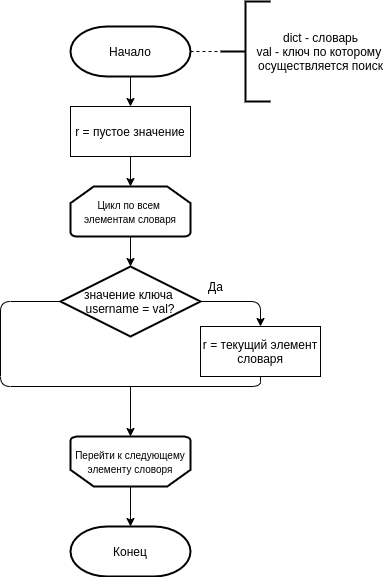
\includegraphics[scale=0.8]{full}}
	\caption{Схема алгоритма полного перебора.}
	%\label{fig:image}
\end{figure}


\begin{figure}[ht!]
	\center{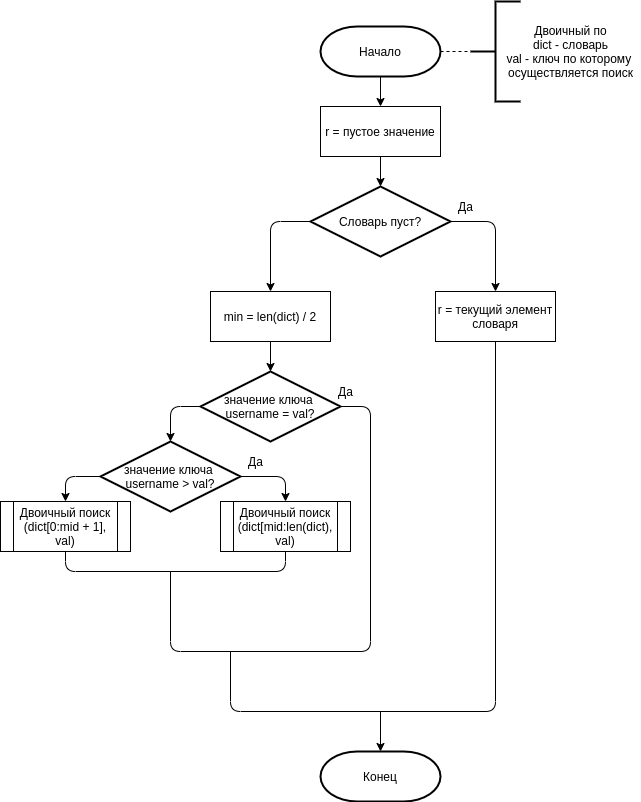
\includegraphics[scale=0.81]{bin}}
	\caption{Схема алгоритма с бинарным поиском.}
	%\label{fig:image}
\end{figure}

\begin{figure}[ht!]
	\center{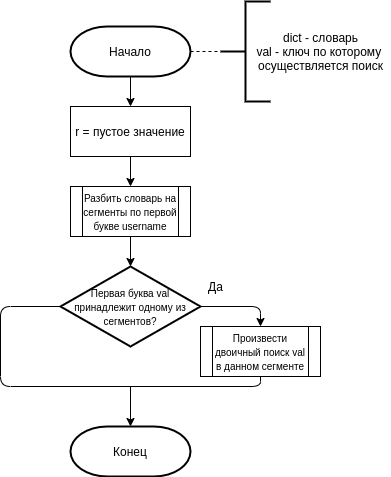
\includegraphics[scale=0.8]{segAnal}}
	\caption{Схема алгоритма с частотным анализом.}
	%\label{fig:image}
\end{figure}

\newpage
\newpage
\section{Описание структуры программного обеспечения}

\begin{figure}[ht!]
	\center{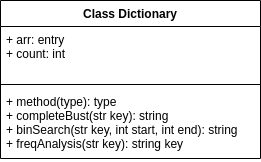
\includegraphics[scale=0.8]{struct}}
	\caption{Структура ПО.}
	%\label{fig:image}
\end{figure}

\newpage
\section{Описание структур данных}

Для реализации данных алгоритмов, введем некоторые типы данных:

\begin{itemize}
	\item entry - тип данных описывающий пару ключ(string) + значение(string); 
	\item segment - тип данных описывающий сегмент частотного анализа первая буква(char) + массив(int) с индексами ключей начинающимися на эту букву
\end{itemize}


\section*{Вывод}

На основе теоритических данных, полученных из аналитического раздела, были построены схемы реализируемых алгоритмов.

Так же, было приведено описание вводимых типов данных.

\newpage
\chapter{Технологическая часть} 

В данном разделе приведены средства реализации, требования к ПО и листинги кода.

\section{Средства реализации}
В качестве языка программирования был выбран с++. Данный язык знаком и предостовляет все необходимые ресурсы.
В качестве среды разработки я использовала Visual Studio Code, т.к. считаю его достаточно удобным и легким.
Visual Studio Code подходит не только для  Windows, но и для Linux, это еще одна причина, по которой я выбрала VS code, т.к. у меня установлена ОС  fedora 34.


\section{Сведенья о модулях программы}

Данноя программа разбита на модули:

\begin{itemize}
	\item main.cpp - файл, содержащий точку входа в программу;
	\item dictionary.cpp - файл, содержащий реализацию алгоритмов поиска в словаре.
\end{itemize}

\section{Реализация конвейера}


\noindent\textrm{Листинг 3.1: Созданные типы данных.}
\begin{lstlisting}[frame=single, numbers=left]
struct entry{
	std::string value;
	std::string key;
} ;

struct segment{
	char first;
	std::vector<int> arrInt;
};
\end{lstlisting}


\noindent\textrm{Листинг 3.2: Функция реализация алгоритма полного перебора.}
\begin{lstlisting}[frame=single, numbers=left]
std::string Dictionary::completeBust(std::string key){
    std::string val = "meh";
    for (int i = 0; i < count; i++){
        if (key == arr[i].key)
            val = arr[i].value;
    }
    return val;
}	
	
\end{lstlisting}

\noindent\textrm{Листинг 3.3: Функция реализация бинарного поиска.}
\begin{lstlisting}[frame=single, numbers=left]
std::string Dictionary::binSearch(std::string key, int start, int end){
    std::string val = "meh";
    if (end - start < 2)
  	{
   	    if (key == arr[start].key)
            return arr[start].value;
        if (key == arr[end].key)
            return arr[end].value;    
        return val;
    }
    int mid = (end - start)/2;
    if (key == arr[mid + start].key)
        return arr[mid + start].value;
    if (key > arr[mid + start].key)
        return binSearch(key, start + mid, end);
    else
        return binSearch(key, start, start + mid);
}
\end{lstlisting}

\noindent\textrm{Листинг 3.4: Функция разделения на сегменты.}
\begin{lstlisting}[frame=single, numbers=left]
void Dictionary::createSeg(){
    int f;
    for (int i = 0; i < count; i++)
    {
        f = arr[i].key[0] - '0';
        seg[f].arrInt.push_back(i);
    }
}
\end{lstlisting}


\noindent\textrm{Листинг 3.5: Функция реализации частотного анализа.}
\begin{lstlisting}[frame=single, numbers=left]
std::string Dictionary::freqAnalysis(std::string key){
    int f = key[0] - '0';
    int size = seg[f].arrInt.size();
    return binSearch(key, seg[f].arrInt[0],
                          seg[f].arrInt[size - 1]);
    return "meh";
}
\end{lstlisting}

\section{Тестирование}

В данном разделе будет приведена таблица с тестами (таблица \ref{table:ref1}).

Тестирование проводилось в словаре, содержащем следущие записи:
\begin{itemize}
	\item key: "номер ОМС"  +  value: "ФИО" .
\end{itemize}	

\begin{table}[ht]
	\centering
	\caption{Таблица тестов}
	\label{table:ref1}
	\begin{tabular}{ | l | l | l |}
		\hline
		Входные данные                        & Пояснение              & Результат    \\ \hline
		0002530407440900 & Первый элемент         & Ответ верный \\ \hline
		5091479945279275              & Средний элемент        & Ответ верный \\ \hline
		9997951582572083                             & Последний элемент      & Ответ верный \\ \hline
		2123566581544639                                & Произвольный элемент   & Ответ верный \\ \hline
		25436523                           & Несуществующий элемент & Ответ верный \\ \hline
		\hline
	\end{tabular}
\end{table}

Все тесты пройдены.


\section*{Вывод}

В данном разделе были реализованны вышеописанные алгоритмы поиска в словаре. Было разработано ПО, удовлетворяющее предьявляемым требованиям. Так же были представлены соответствующие листинги с кодом программы. А так же проведено тестирование разработанного ПО.

\newpage
\chapter{Исследовательская часть} 

В данном разделе будет произведено измерение временных характеристик.

\section{Технические характеристики}


Технические характеристики устройства на котором выполнялось исследование:
\begin{itemize}
	\item процессор Intel® Core™ i5-10210U CPU @ 1.60GHz × 8;
	\item память 15.3 GiB;
	\item операционная система Fedora 34 (Workstation Edition) 64-bit.
\end{itemize}

%Исследования проводились на ноутбуке включенном в сеть электропитания. Во время тестирования ноутбук был нагружен приложениями окружения рабочего стола, а так же системой тестирования.



\section{Временные характеристики}

Так как поиск в словаре считается короткой задачей, воспользуемся усреднением массового эксперимента.
Для этого сложим результат работы алгоритма n раз (n >= 10), после чего поделим на n.
Тем самым получим достаточно точные характеристики времени.
Сравнение произведем при n = 1000.

\begin{figure}[ht!]
	\center{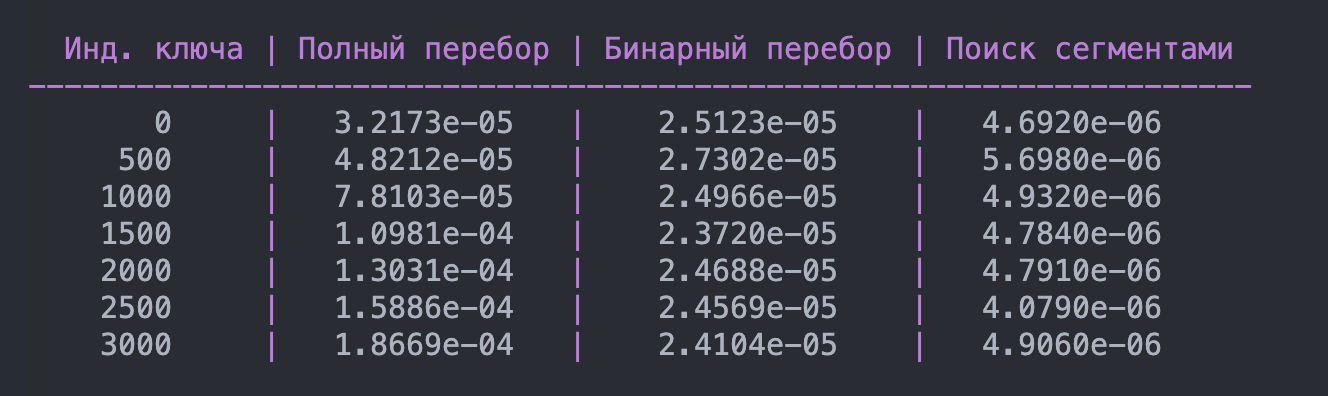
\includegraphics[scale=0.75]{time3}}
	\caption{Время работы алгоритмов.}
	%\label{fig:image}
\end{figure}


\begin{figure}[ht!]
	\center{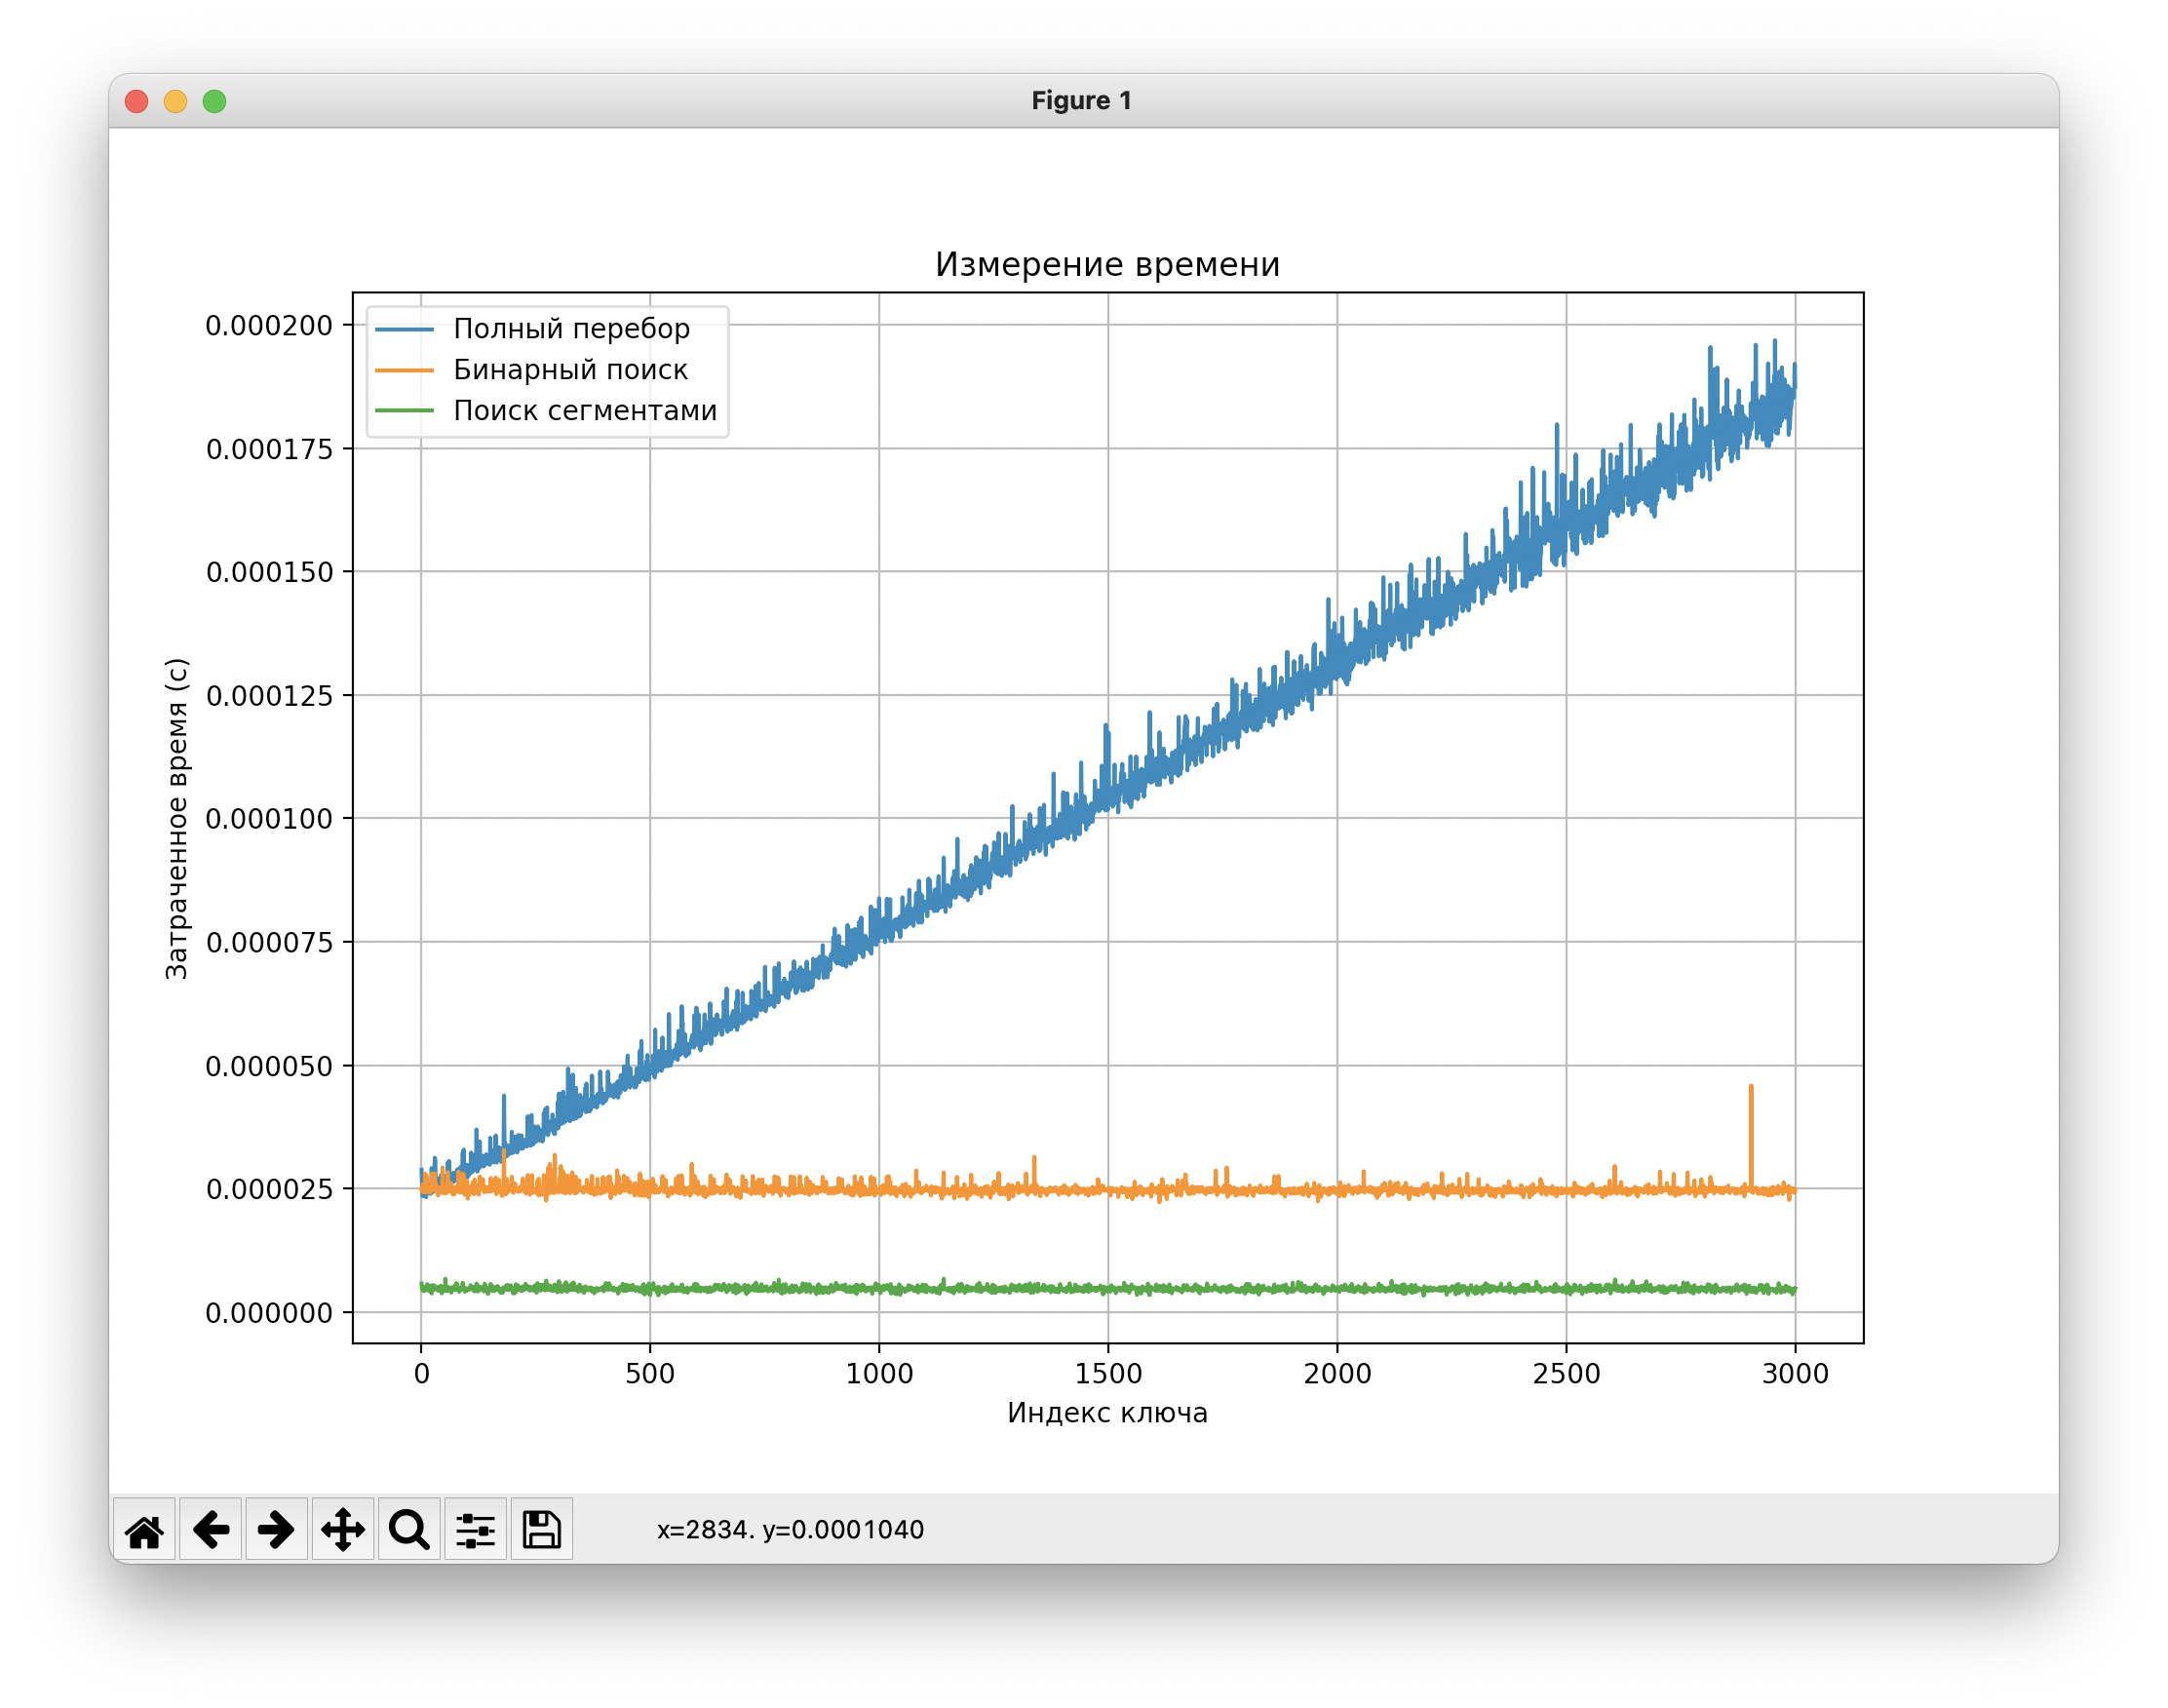
\includegraphics[scale=0.4]{graph_time}}
	\caption{Зависимость времени паботы алгоритмов поиска от индекса клюса.}
	%\label{fig:image}
\end{figure}


\newpage
\begin{itemize}
	\item представлен результат поиска первого значения.
	Выигрыш алгоритма поиска полным перебором обосновывается тем, что он тратит
	лишь одно сравнение для того, чтобы найти первый ключ, в том время, когда
	бинарный поиск затрачивает гораздо больше сравнений.
	Частичный анализ работает чуть медленнее, так как ему нужно
	произвести дополнительное сравнение первых букв.
	\item представлен результат поиска среднего значения. Выйгрыш бинарного поиска в том что он находит середину за одну итерацию.
	\item приведено сравнение времени выполнения
	трех алгоритмов для поиска последнего значения.
	По результатам эксперимента видно, что поиск полным перебором
	затрачивает больше всего времени, т.к. он последовательно обходит
	все элементы, в то время, как остальные два алгоритма выполняют
	поиск значительно быстрее.
	\item представлен результат поиска произвольного ключа.
	Алгоритм полного перебора работает медленнее всех.
	\item произведено аналогичное сравнение, только в качестве искомого ключа
	взят несуществующий. Аналогично поиск полным перебором
	затрачивает больше всего времени по вышеописанной причине.
\end{itemize}


\section{Колличество сравнений при работе алгоритмов}

Для каждого алгоритма был проведён анализ по количеству сравнений для нахождения каждого ключа в словаре. Были составлены по две гистограммы для всех алгоритмов поиска (ключи расположены в том же порядке, как и в словаре, и когда ключи отсортировнны в порядке убывания).


\begin{figure}[h]
	\centering
	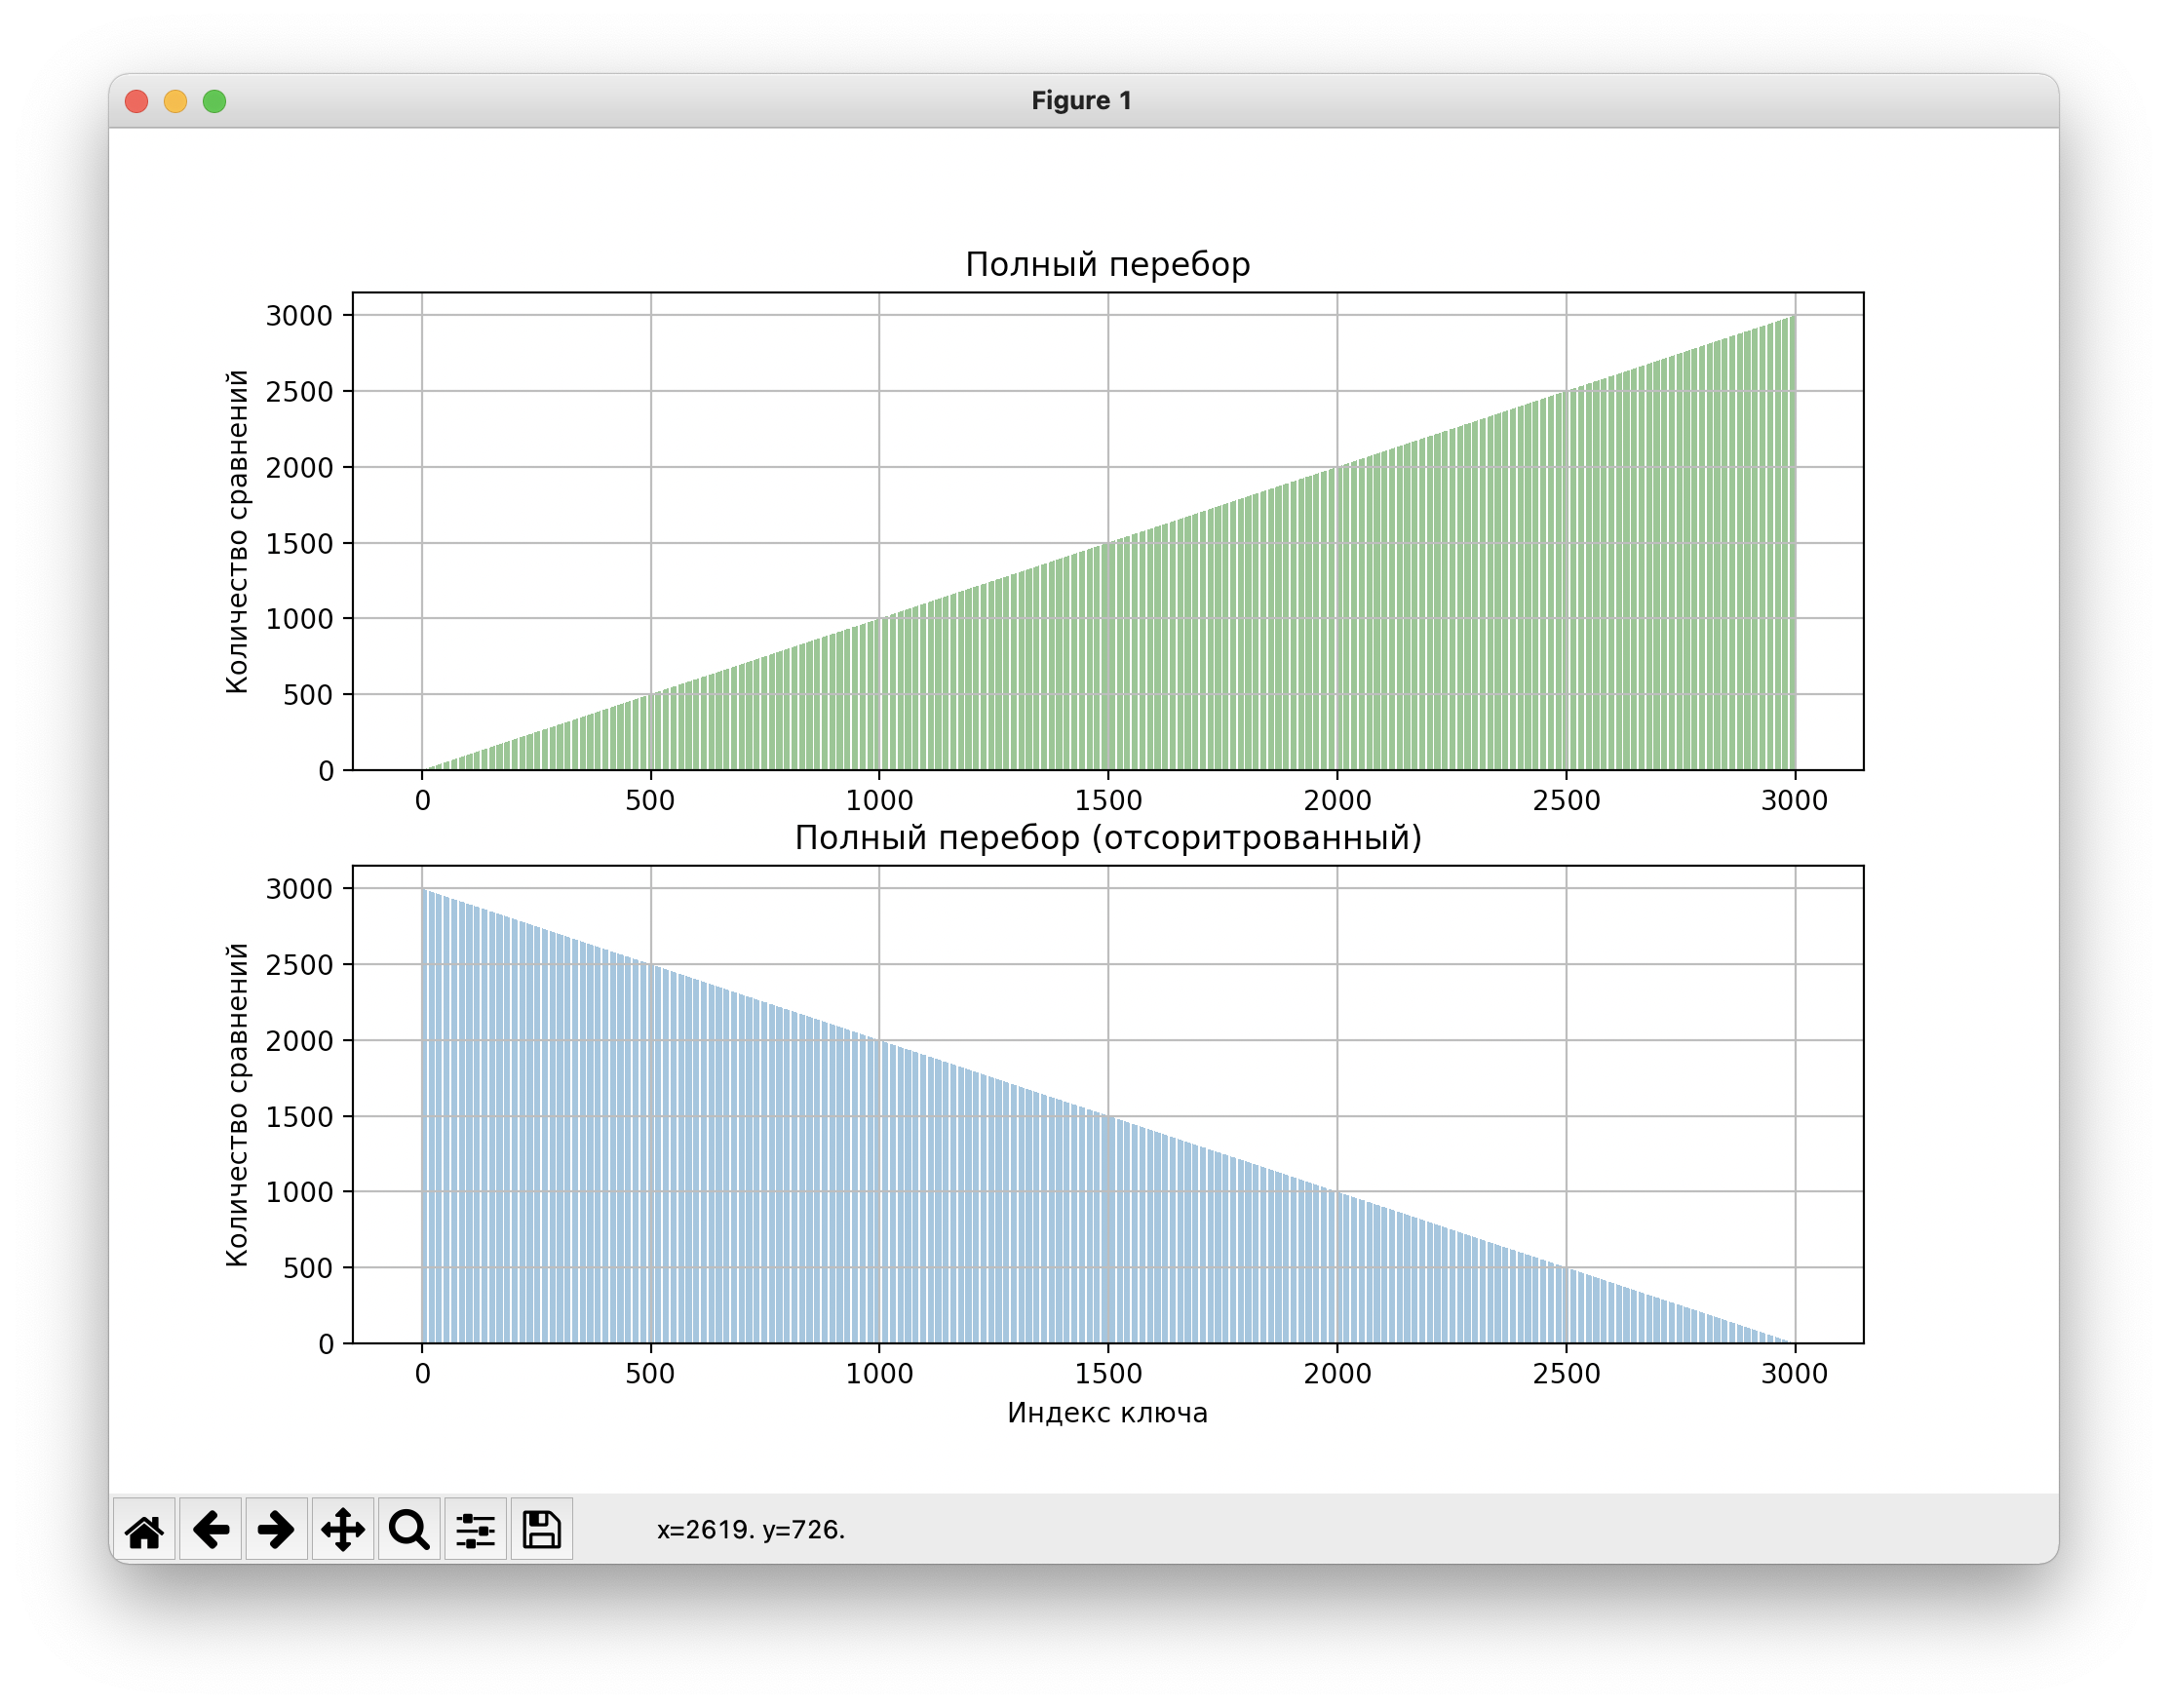
\includegraphics[scale=0.45]{graph_full_search.png}
	\caption{Кол-во сравнений при поиске ключа в словаре (полным перебором)}
	\label{fig:graph_full_search}
\end{figure}

\clearpage

\begin{figure}[h]
	\centering
	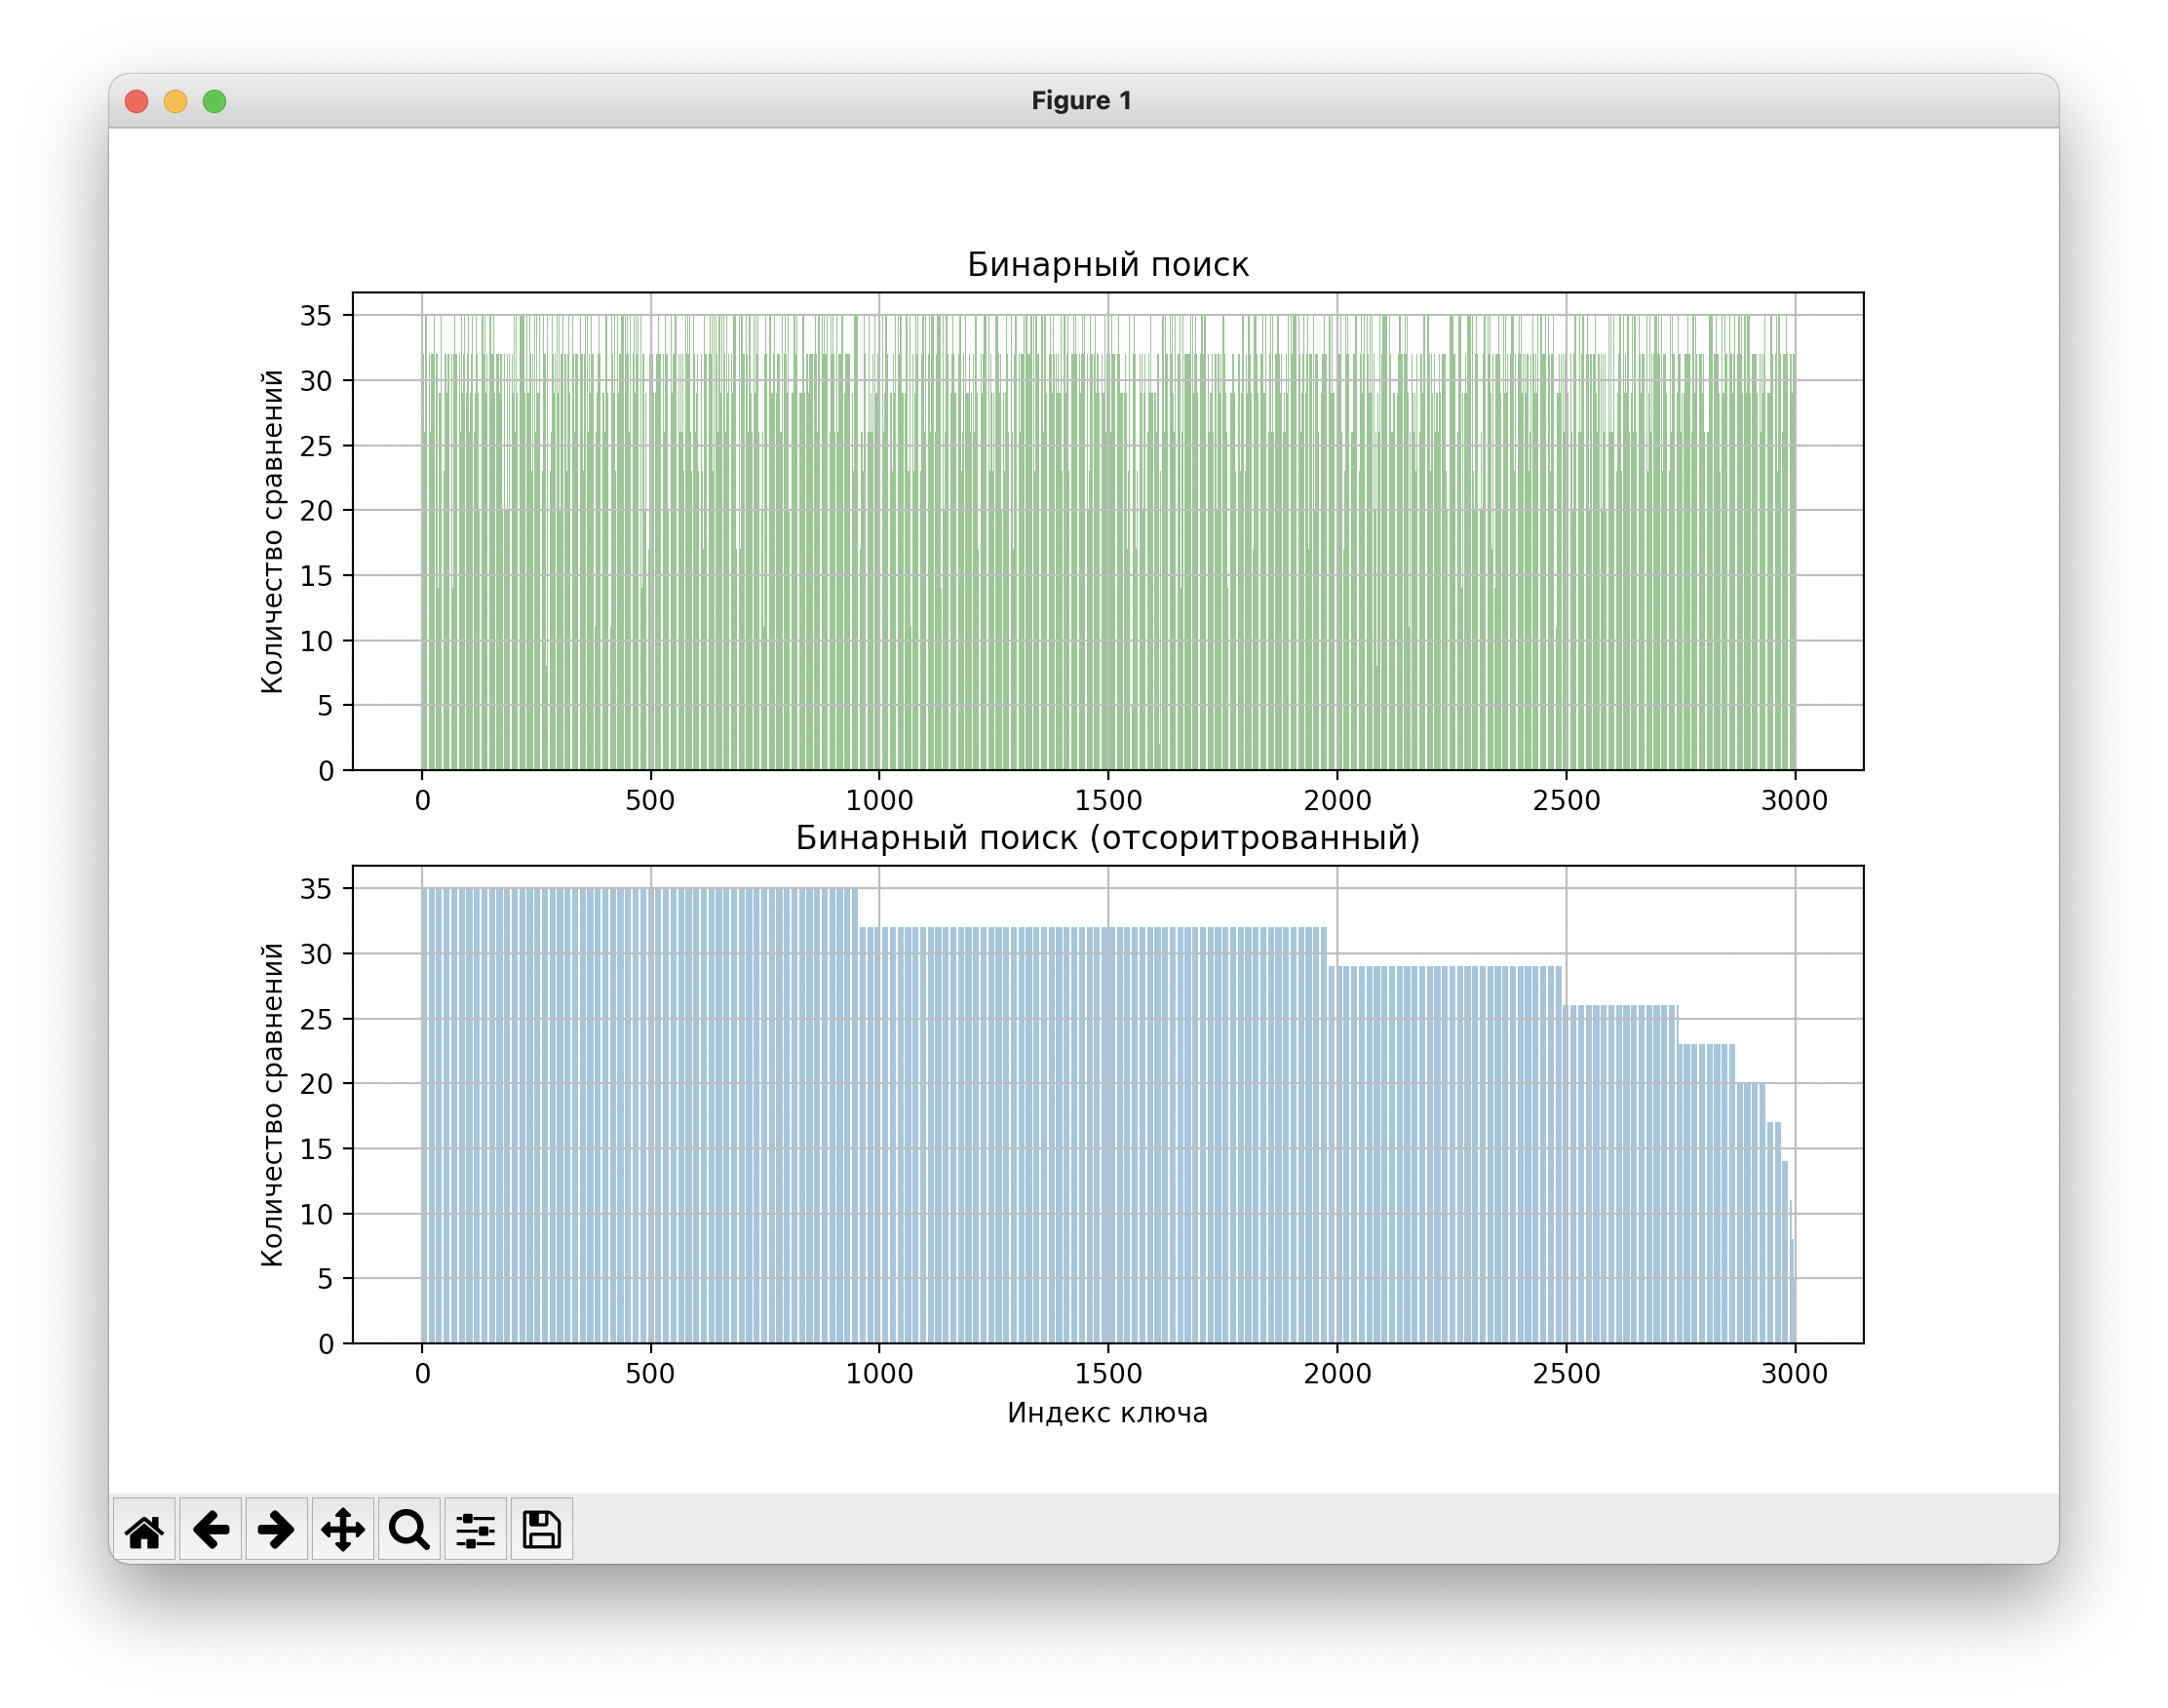
\includegraphics[scale=0.45]{graph_binary_search.png}
	\caption{Кол-во сравнений при поиске ключа в словаре (бинарным поиском)}
	\label{fig:graph_binary_search}
\end{figure}

\clearpage

\begin{figure}[h]
	\centering
	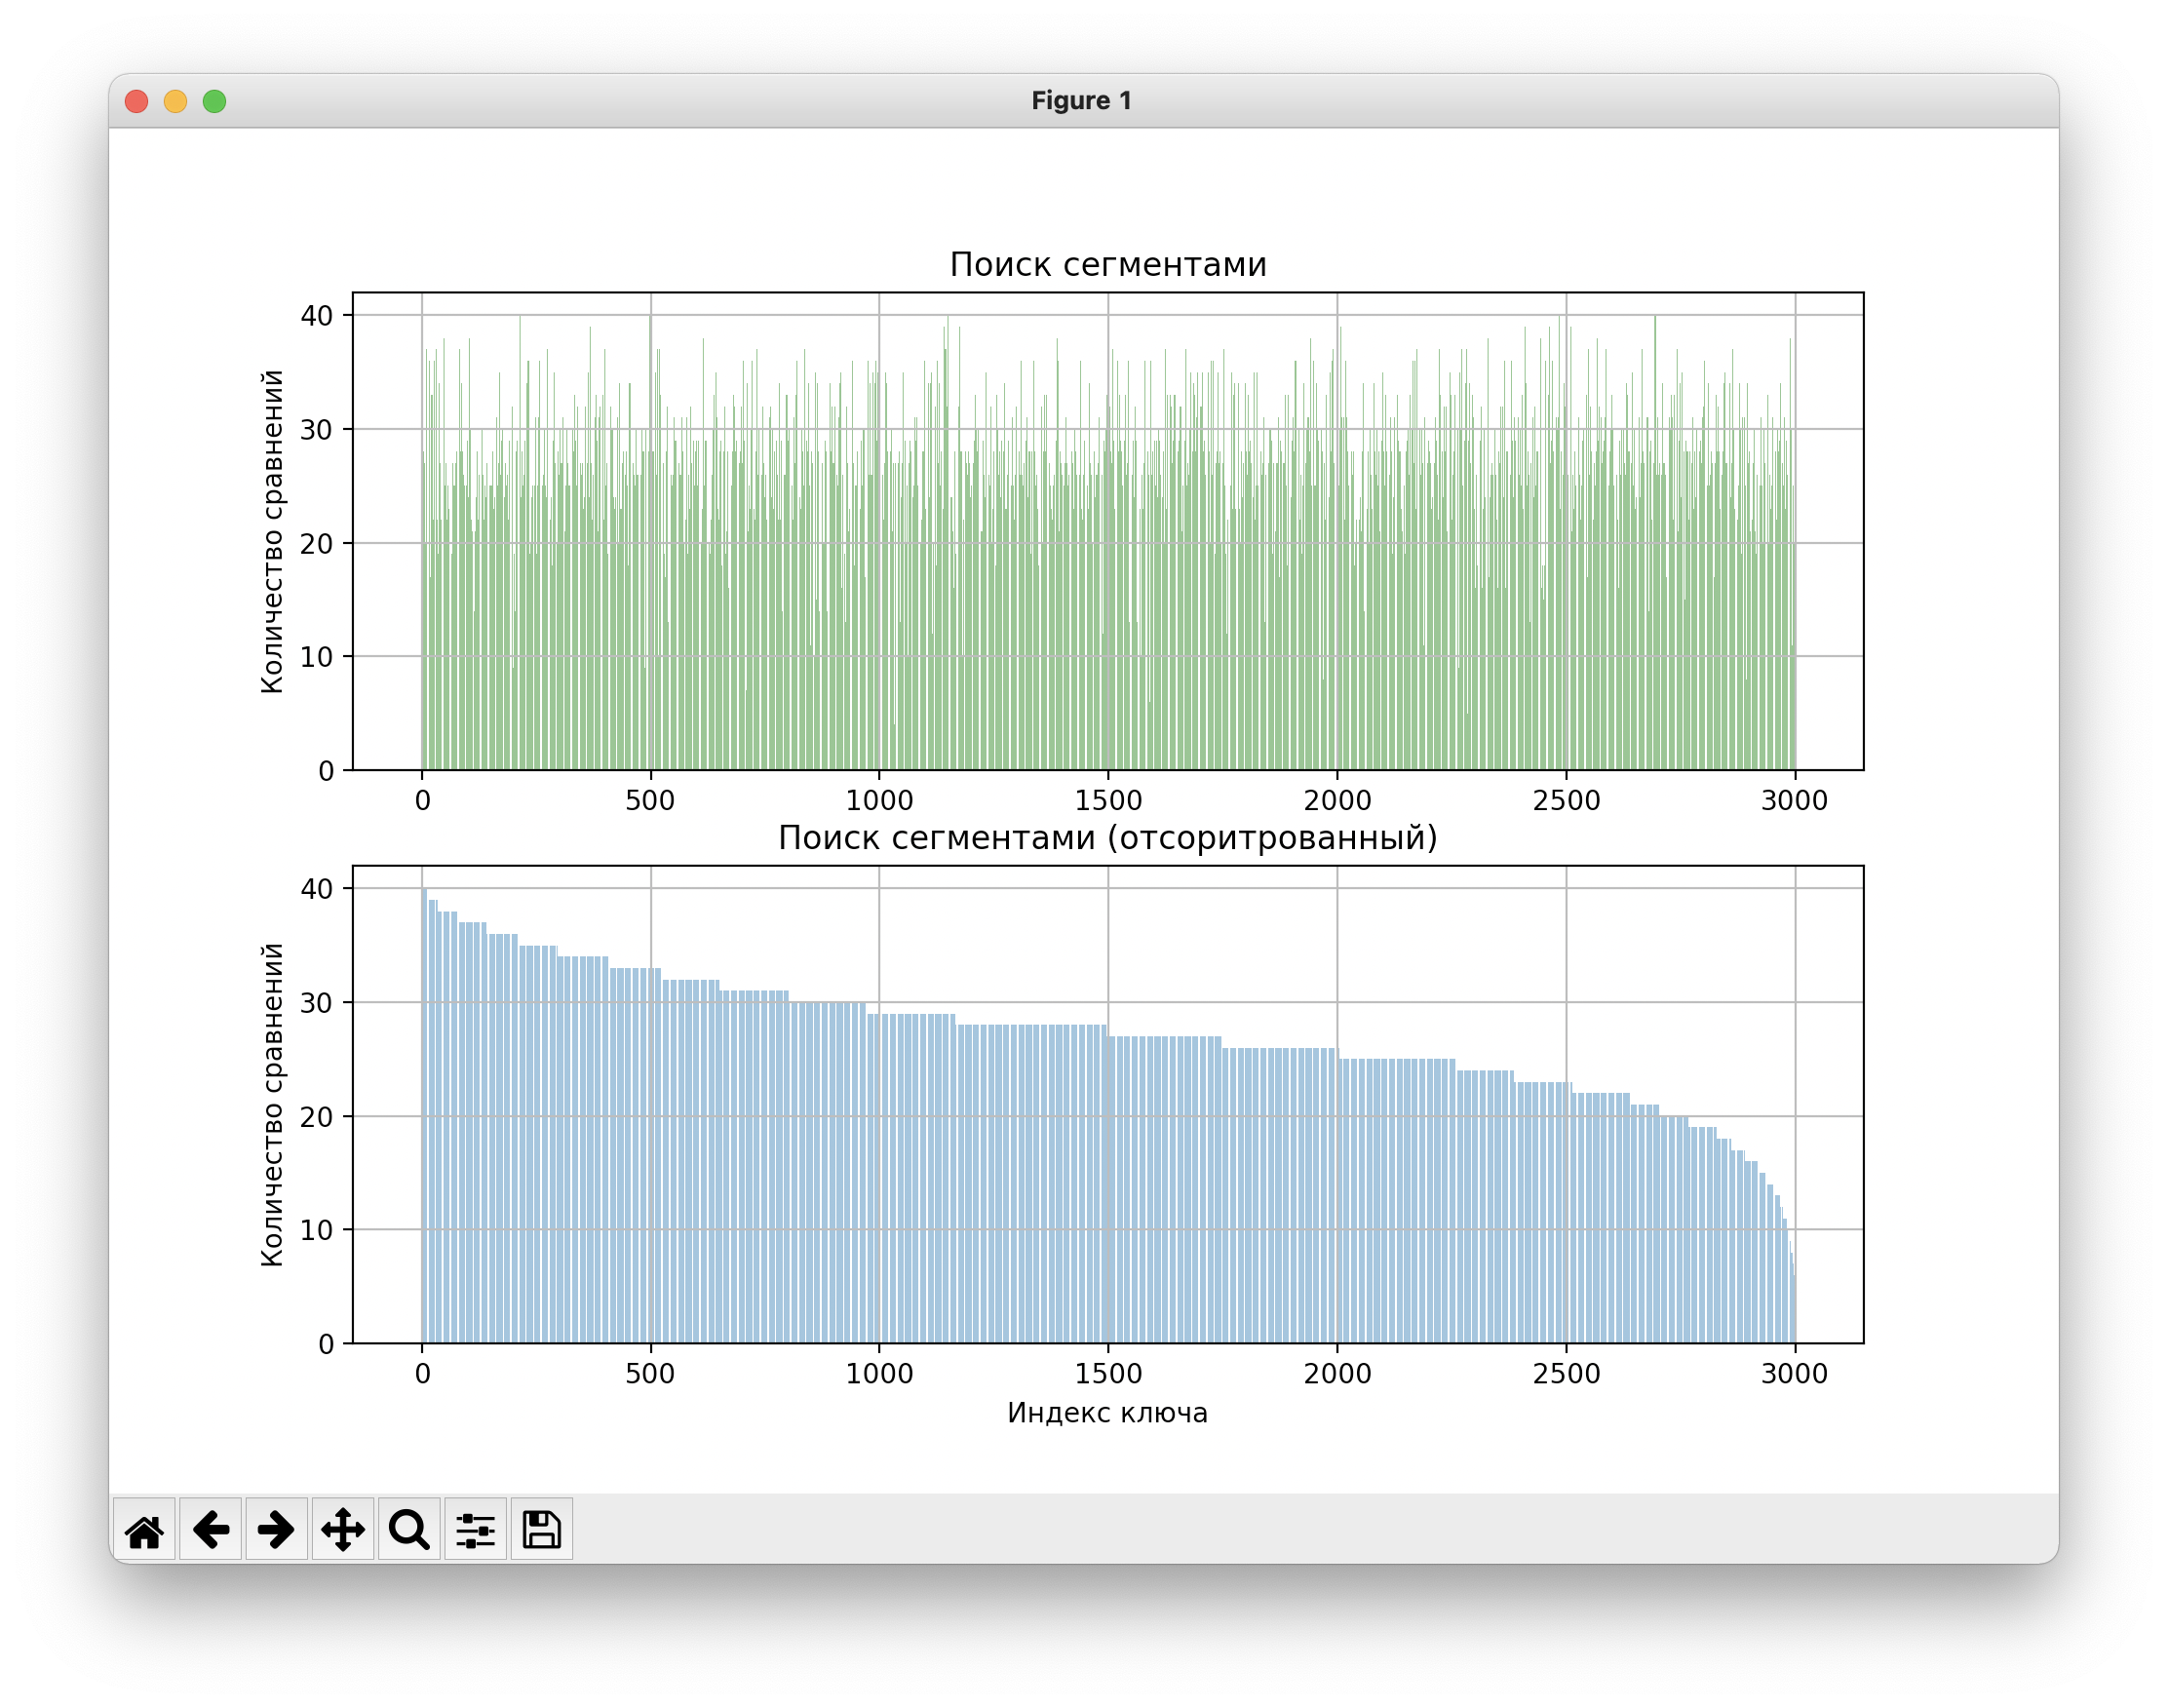
\includegraphics[scale=0.45]{graph_segment_search.png}
	\caption{Кол-во сравнений при поиске ключа в словаре (поиском сегментами)}
	\label{fig:graph_segment_search}
\end{figure}




\section{Вывод}

В данном разделе было произведено сравнение трех алгоритмов.
По результатам исследования было доказано, что алгоритм полного перебора
в основном работает медленнее всех, за исключением, когда ключ лежит достаточно
близко к началу.


\newpage
\chapter*{Заключение}
\addcontentsline{toc}{chapter}{Заключение}
	
В данной лабораторной работе были изучены алгоритмы поиска по ассоциативному словарю.

Среди рассмотренных алгоритмов наиболее эффективным по времени является алгоритм бинарного поиска. Однако при больших размерностях входных массивов алгоритм бин поиска становиться менее эффективным, чем алгоритм частотного анализа. Поэтому, при большом числе элементов входного массива стоит использовать данный алгоритм.

В рамках лабораторной работы цель достигнута и выполнены следующие задачи:

\begin{itemize}
	\item исследованы алгоритмы поиска по словарю;
	\item приведены схемы рассматриваемых алгоритмов;
	\item проведены тестирование работы алгоритмов в лучшем, худшем и произвольном случае;
	\item проведены замеры процессорного времени работы алгоритмов поиска по словарю для каждого ключа и для отсутствующего ключа, вывести минимальное, максимальное и среднее время поиска ключа;
	\item сделан вывод о проделанной работе и описать в отчете.
\end{itemize}
	
	
\newpage
\renewcommand\bibname{Список литературы}
\addcontentsline{toc}{chapter}{Список литературы}
\makeatletter % список литературы
\def\@biblabel#1{#1. }
\makeatother
\begin{thebibliography}{2}
	\bibitem{analyse_info} Дж. Макконнел. Анализ алгоритмов. Активный обучающий подход. -- М.: Техносфера, 2017. -- 267с.
	\bibitem{anatyse_info}Основы программирования на языках Си и C++ для начинающих[Электронный ресурс]. Режим доступа: http://cppstudio.com/ (дата обращения 10.10.2021)
	\bibitem{analyse_info}LINUX.ORG.RU - Русскоязычная информация о ОС Linux[Электронный ресурс] Режим доступа://www.linux.org.ru/(дата обращения 25.10.2021)
	\bibitem{analyse_info}  Документация языка C++ 98 [Электронный ресурс], режим доступа: http://www.open-std.org/JTC1/SC22/WG21/ (дата обращения 10.12.2021)
	\bibitem{analyse_info}Кнут Д. Э. Искусство программирования. Том 3. Сортировка и поиск = The Art of Computer Programming. Volume 3. Sorting and Searching / под ред. В. Т. Тертышного (гл. 5) и И. В. Красикова (гл. 6). — 2-е изд. — Москва: Вильямс, 2007. — Т. 3. — 832 с. — ISBN 5-8459-0082-1.
	
\end{thebibliography}

\end{document}